\section{Complete tables and figures}\label{sup:results}

% The paper cites these subsections by number (S4.1 to S4.8): keep their order.

All tables and figures of this section are generated from the result files of the repository
(\code{results/battery.csv}, \code{results/terms.csv}, \code{results/stats.json},
\code{results/timing.csv}) by the same script as those of the paper
(\code{tools/paper\_results.py}). The methods of the library are shown by their runs on Chrono.
Abbreviations: Gon (\law{gonthier}), G18 (\law{gonthier-thesis}), Dis (\law{distributed}), Dis-v
and Dis-1 (its vertex and one-point friction rules), PCM; Dr-h and Dr-p (Drake hydroelastic and
point), Ch-S and Ch-N (Chrono SMC and NSC), Mj-s and Mj-d (MuJoCo soft and default). Errors are
in percent of the reference.

\subsection{The runs, and those without an error value}

The main matrix was run on \result{battery/date} with the code of commit
\result{battery/commit}; the friction quadratures and \law{pcm} were added at commit
\result{battery/commit-baselines}, after \result{battery/spot-runs} runs spread over the
scenarios reproduced the main matrix (largest relative difference \result{battery/spot-diff}).
The runs of the matrix add up to \result{battery/cpu-hours} hours of wall-clock time. Every run
ends with one of four statuses: \emph{ok}; \emph{nan}, when it finished but a quantity that the
reference fixes was not produced; \emph{timeout}; and \emph{failed}, when the engine stopped
with an error. Of the \result{battery/runs} runs, \result{battery/ok} finished with an error
value and \result{battery/failed} did not (\result{battery/nan} nan, \result{battery/timeout}
timeout, \result{battery/crashed} failed): the two laws have \result{status/laws/notok} such
run, the native models \result{status/natives/notok} and the other methods of the library
\result{status/baselines/notok} (Table~\ref{tab:status}). Their causes, where known: \scn{tip}
with every point-contact model (a tall box on stiff points tips at the rigid angle, which the
ramp of the scenario, designed for the lower angle of the foundation, never reaches);
\scn{disk} and \scn{contensou} with Chrono SMC and Drake point, and \scn{cone} with the latter
(a flat face held by one to three points wobbles and never meets the stop criterion);
\scn{oblique} and \scn{restitution} with Chrono NSC and three isolated runs of Chrono NSC (not
diagnosed); \scn{tower} and the smallest steps of \scn{stack} and \scn{massratio} with Drake
hydroelastic (the time limit); and \scn{massratio} with \law{gonthier-thesis} on Drake and
MuJoCo and one run of \law{gonthier} on Drake (beyond the stability limit of the explicit
coupling; the same runs on the other engines finish with errors above 1000\,\%).

\begin{table}[!htbp]
\caption{Runs that did not finish with an error value, by method and status}
\label{tab:status}
\generatedtable{status}
\end{table}

\subsection{The same law on three engines}

Table~\ref{tab:independence} and Fig.~\ref{fig:independence} compare the error of each method
of the library on the three engines. Relative to the error itself the largest difference of
\law{distributed} is \result{ind/distributed/maxrel}, in a scenario whose error is below
1\,\%, and at the smallest step the largest difference is
\result{ind/distributed/maxabs/dt0.1}. In \scn{massratio}, which is lost, the three engines also
agree in relative terms for the two laws, while the lost runs of \law{gonthier-thesis} and
\law{pcm} differ more.

\begin{table}[!htbp]
\caption{Largest spread of the error of each method of the library over the three engines,
base variant. Held: scenarios with an error below 100\,\% on every engine; lost: the others,
left out of the next columns. pp: percentage points}
\label{tab:independence}
\generatedtable{independence}
\end{table}

\begin{figure}[!htbp]
\centering
\generatedfigure[width=0.85\linewidth]{independence}
\caption{Error [\%] of the two laws on Drake and on MuJoCo against their error on Chrono, every
scenario, base variant. The point at the upper right is \scn{massratio}, which is lost on the
three engines}
\label{fig:independence}
\end{figure}

\subsection{Errors by scenario; the development set and the second set}\label{sup:errors}

The errors by class are Tables~3 to~5 of the paper; Figs.~\ref{fig:heatmap-A}
and~\ref{fig:heatmap-BC} show the same errors as heat maps, and
Table~\ref{tab:errors-heldout} those of the second set alone.

\begin{figure}[!htbp]
\centering
\generatedfigure{heatmap_A}
\caption{Class A: error [\%] of every method on every scenario, base variant, logarithmic colour
scale; methods of the library on Chrono. Hatched cells are runs without an error value (nan;
t/o: time limit)}
\label{fig:heatmap-A}
\end{figure}

\begin{figure}[!htbp]
\centering
\generatedfigure{heatmap_BC}
\caption{Classes B and C: error [\%], base variant; methods of the library on Chrono. Class C
compares only the methods that are a Winkler foundation}
\label{fig:heatmap-BC}
\end{figure}

\begin{table}[!htbp]
\caption{Second set: error [\%] of each method, base variant}
\label{tab:errors-heldout}
\generatedtable{errors_heldout}
\end{table}

The development set has \result{battery/dev} scenarios, written while the laws were being
developed; the laws were changed in response to them, and every change was general (no scenario
has a constant of its own). The \result{battery/heldout} scenarios of the second set were
written, with their references, parameters and error terms, before any contact law was run on
them; one of them, \scn{massratio}, was written to find the limit of the explicit coupling. No
law, parameter or engine setting was changed for them before their first run, and none of them
was changed after it except to add recorded quantities and to let one of them run on every
engine. Three changes to the laws lie between that first run and the battery: the bounds on the
terms proportional to the load (Section~\ref{sup:bounds}) and the bristle on the material slip,
both adopted because of that first run, and the treatment of the seams with the damping along
the pair normal and the exact clamp, prompted by the development set and merged after it. The
errors of the two laws on the second set are therefore not out-of-sample errors, and the set is
not held out; only its first run was (the result files of the repository keep the label
``heldout'' for it). Table~\ref{tab:heldout-first} sets the errors of that first run next to
the ones reported. In the first run the two laws lost \scn{tower} and \scn{massratio},
\law{gonthier} with the bristle of the 2018 thesis did not hold the block of \scn{wedge}
(\result{first/wedge/gonthier}), and \law{distributed} gained energy in \scn{energy}
(\result{first/energy/distributed}). \scn{turntable} got worse for \law{distributed} (from
\result{first/turntable/distributed} to \result{err/turntable/distributed}), because the
corrected damping has the rolling resistance that the earlier one lacked by accident. Of the
\result{battery/n/A-heldout} scenarios of class A in the second set, \law{distributed} is within
5\,\% in \result{passn/A/distributed/5/heldout} and \law{gonthier} in
\result{passn/A/gonthier/5/heldout}; in the development set they are within 5\,\% in
\result{passn/A/distributed/5/dev} and \result{passn/A/gonthier/5/dev} of
\result{battery/n/A-dev}.

\begin{table}[!htbp]
\caption{Second set, the two laws: error [\%] in the first run of the set, made before the
changes that it caused (single runs on Chrono at commit \code{4d5a0da}, transcribed from the
history of the repository; they cannot be regenerated from the result files), and in the
battery reported in the paper}
\label{tab:heldout-first}
\generatedtable{heldout_first}
\end{table}

\subsection{Counts within thresholds, and the band}

Table~\ref{tab:pass} counts the scenarios that each method solves within 1, 5 and 20\,\%, and
Table~\ref{tab:band} the position of each method against the band of admissible pressure
distributions of class B. For \scn{ring} and \scn{cone}, whose bands have a side of zero width,
every run is undetermined or outside.

\begin{table}[!htbp]
\caption{Number of scenarios within 1, 5 and 20\,\% of their reference, base variant. Runs
without an error value count as not within. Reduced: class A without \scn{bowl}, \scn{trough},
\scn{turntable} and \scn{edge}}
\label{tab:pass}
\generatedtable{pass_rates}
\end{table}

\begin{table}[!htbp]
\caption{Class B: number of scenarios in which a method is inside the band of admissible
pressure distributions, outside it, undetermined (the error exceeds the narrow side of the band
only, and its sign was not recorded) or without a stop time; base variant}
\label{tab:band}
\generatedtable{band}
\end{table}

Figure~\ref{sup:fem} plots the pressure of the finite-element reference of the paper's
Section~5.4 against the distributions of the band of \scn{disk} and \scn{bearing}.

\begin{figure}[!htbp]
\centering
% Written by tools/fem/run.py (results/fem/figures/), not by tools/paper_results.py.
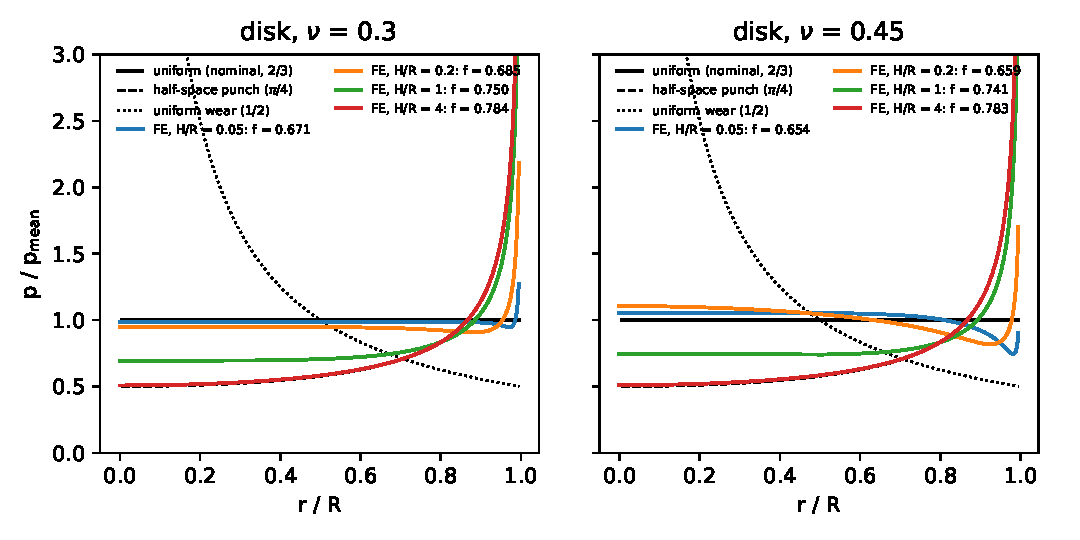
\includegraphics[width=0.9\linewidth]{../results/fem/figures/disk_pressure.pdf}\\[2pt]
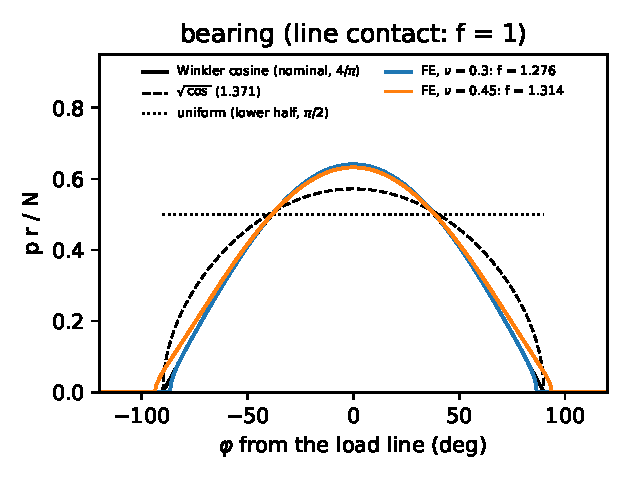
\includegraphics[width=0.55\linewidth]{../results/fem/figures/bearing_pressure.pdf}
\caption{Pressure of a linear-elastic support computed by finite elements (Section~5.4 of the
paper) against the distributions of the band. Top: \scn{disk}, layers of several thicknesses
$H/R$ under a rigid flat punch, for $\nu=0.3$ and $0.45$. Bottom: \scn{bearing}, plane-strain
sleeve around a rigid journal}
\label{sup:fem}
\end{figure}

\subsection{The friction quadratures on the battery}

Table~\ref{tab:ablation} compares \law{distributed} with its two quadrature variants and with
\law{pcm} on the meshes of the battery. In \scn{contensou} the closed form has
\result{err/contensou/distributed} against \result{err/contensou/vertex} and
\result{err/contensou/centroid}. In \scn{ring}, whose centre of rotation is outside the face,
the battery's own triangulation already gives \result{tri/ring/spin/quads/64/centroid/moment}
and \result{tri/ring/spin/quads/64/vertex/moment} in the experiment on one face, and the three
rules agree in the battery. Over class A the ratio of the errors of \law{distributed} to those
of its vertex variant is \result{robust/distributed-vs-vertex/A/full} with
\result{robust/distributed-vs-vertex/A/ties} ties in \result{robust/distributed-vs-vertex/A/n}
units, the one unit that differs being the cut ground. The battery's errors are stop times and
combine the two sides of the contact, so they are not the torque errors of the experiment on
one face (\code{tools/ablation\_triangulation.py}). The cost of a quadrature on a remeshed face
at equal accuracy, through the geometry of the larger number of polygons, was not measured.
\law{pcm}, even with the exact contact surface lent to it, has the error of its one-point
friction on the battery's spinning flat contacts and depends on the cut, both of which a finer
mesh of the flat faces would reduce; it cannot hold a body still (\scn{push}, \scn{wedge},
\scn{tip}, \scn{stack}, \scn{tower}), which no mesh changes; and it is the better of the two on
curved conforming contact (\result{err/bearing/pcm} against \result{err/bearing/distributed} in
\scn{bearing}, \result{err/journal/pcm} against \result{err/journal/distributed} in
\scn{journal}).

\begin{table}[!htbp]
\caption{The battery, on its own meshes (flat caps: fans from a rim vertex; grounds: two
triangles per face): error [\%] of the distributed law with the closed-form friction, with the
vertex rule and with the one-point rule, and of the per-face foundation, on the flat spinning
contacts under refinement of the curved meshes (1\,ms) and on the ground cut into pieces}
\label{tab:ablation}
\generatedtable{ablation}
\end{table}

\subsection{Convergence with the step and the mesh}

Table~\ref{tab:convergence} classifies every series by the slope of the logarithm of the error
against the logarithm of the step or of the mesh size as converging, flat (a slope within
$\pm0.2$, or every error below $2\times10^{-3}$), diverging, non-monotone or failed.
Figures~\ref{fig:convergence-dt} and~\ref{fig:convergence-mesh} show the error against the step
and the number of segments in selected scenarios. A flat step series is evidence about the law
as given only where the step bounds of Section~\ref{sup:bounds} are inactive; where they act
(\scn{tower}, \scn{massratio}, \scn{stack}), the applied parameters change with the step.

\begin{table}[!htbp]
\caption{Convergence series by method: number of scenarios in which the error converges
(conv.), stays flat, is not monotone (n-m.), diverges (div.) or a run of the series did not
finish (fail.), with the step (2 to 0.1\,ms) and with the mesh (32 to 128 segments)}
\label{tab:convergence}
\generatedtable{convergence}
\end{table}

\begin{figure}[!htbp]
\centering
\generatedfigure{convergence_dt}
\caption{Error [\%] against the time step in six scenarios. Errors above 3000\,\% are drawn at
that value; a missing point is a run without an error value. Chrono SMC is not shown: its
backend sub-steps}
\label{fig:convergence-dt}
\end{figure}

\begin{figure}[!htbp]
\centering
\generatedfigure{convergence_mesh}
\caption{Error [\%] against the number of segments per turn of the curved meshes in six
scenarios, at 1\,ms}
\label{fig:convergence-mesh}
\end{figure}

\subsection{The stiffness series and the energy measure}

Table~\ref{tab:stiffness} and Fig.~\ref{fig:stiffness} show the effect of a tenfold stiffer
foundation. On class A the error of \law{distributed} falls in \scn{edge}
(\result{err/edge/distributed/dt0.2} to \result{err/edge/distributed/stiff}), \scn{turntable},
\scn{bowl}, \scn{trough}, \scn{billiard}, \scn{oblique} and \scn{journal}, and rises in
\scn{cylinder} and in \scn{massratio}. On the flat \scn{disk} the errors of the two laws rise
(\law{gonthier}: \result{err/disk/gonthier/stiff}) and those of Drake hydroelastic and
\law{pcm} do not (\result{err/disk/hydro/stiff}, \result{err/disk/pcm/stiff}); in the
diagnostic runs behind the flutter condition of the paper the rocking and vertical modes had
$K\,w\,\dt^2$ of 0.08 at 0.2\,ms, and the tilt saturated at about 65 times its amplitude at
$K$. In the diagnostic run of \scn{cone} at $10K$ the frustum wobbled by 0.065\,rad and climbed
out of its seat, at an error that did not depend on the step.
% Diagnostic single runs on Chrono, docs/research/anomalies.md §1.

\emph{The energy measure.} Over the perturbed starts the measure of \scn{energy} covers
\result{pertrange/energy/gonthier/range} for \law{gonthier},
\result{pertrange/energy/pcm/range} for \law{pcm} and
\result{pertrange/energy/distributed/range} for \law{distributed}. For \law{gonthier} it falls
to \result{err/energy/gonthier/mesh128} with 128 segments, and in diagnostic runs at the base
step with ten times the stiffness, where the penetration and the energy that it stores are
smaller, it was 0.02 to 0.03\,\% for the two laws; in the diagnostic run at the base stiffness
the energy never exceeded its start by more than 1.8\,\%.
% 0.016 %, 0.03 % and 1.8 %: single diagnostic runs, docs/research/anomalies.md §2
The single run made when the scenario was written gave \result{first/energy/gonthier} for
\law{gonthier}; since the runs are deterministic, something changed the nominal trajectory
between that commit and the battery, and which change it was has not been identified (it was
not bisected).

\begin{table}[!htbp]
\caption{Error [\%] at the stiffness of the scenario and at ten times that stiffness
($K \to 10K$), both at 0.2\,ms, classes A and B}
\label{tab:stiffness}
\generatedtable{stiffness}
\end{table}

\begin{figure}[!htbp]
\centering
\generatedfigure{stiffness}
\caption{Error [\%] of the distributed law and of Drake hydroelastic at the stiffness of each
scenario and at ten times that stiffness, at 0.2\,ms. The dotted line separates class A from
class B; a cross is a run without an error value}
\label{fig:stiffness}
\end{figure}

\subsection{Cost}\label{sup:cost}

Table~\ref{tab:cost} gives the cost of every method and Fig.~\ref{fig:work-precision} sets it
against the share of scenarios solved within 5\,\%. The timings are those of
\result{cost/source}, with the code of commit \result{battery/timing-commit} on
\result{battery/timing-date}; the two friction quadratures were not timed, and Chrono SMC is
sub-stepped by its backend. Drake hydroelastic did not finish \scn{tower} within the limit of
the timing pass, so \scn{tower} is not in its median or its maximum. The only figure for that
run is of another kind and is not comparable with the timings: in the accuracy pass, on a
loaded machine, it used its hour of time limit without finishing, which puts its cost above
\result{cost/bound/tower-hydro} times real time, a lower bound that the load inflates by an
unknown factor. The costs of the native models are those of our configurations at the step of
the battery, not at the larger steps that implicit solvers allow.

\begin{table}[!htbp]
\caption{Wall-clock time over simulated time across the scenarios, base variant
(\result{cost/label}). Runs: scenarios timed; Drake hydroelastic did not finish \scn{tower}}
\label{tab:cost}
\generatedtable{cost}
\end{table}

\begin{figure}[!htbp]
\centering
\generatedfigure{work_precision}
\caption{Share of class A and B scenarios within 5\,\% against the wall-clock time over the
simulated time (\result{cost/label}). Marker: median over the scenarios; bar: 10th to 90th
percentile}
\label{fig:work-precision}
\end{figure}
